% http://guitarpenguin.is-programmer.com/posts/48869.html
% fix tex4ht:
% https://tex.stackexchange.com/questions/185349/error-using-pgfsysdriver-with-tex4ht-only-shows-up-with-texlive-2014-ok-with-t

\documentclass{article}
\def\pgfsysdriver{pgfsys-tex4ht.def}
%There is specialized output driver for use with tex4ht in Tikz. Using it, diagrams are saved in SVG.
\usepackage{tikz}
\usepackage{pgf}
\usepackage{hyperref}
\usepackage{xcolor}
\usetikzlibrary{arrows.meta}

\usetikzlibrary{automata}
\usetikzlibrary{positioning,chains,fit,shapes,calc}
\usetikzlibrary{arrows,shadows,trees}

\definecolor{linkcolor}{RGB}{64, 112, 160}

\begin{document}
\begin{tikzpicture}[->,>=stealth',node distance=1cm]

  \tikzstyle{block}=[fill=white, draw={rgb:red,225;green,228;blue,229}, text={rgb:red,64;green,112;blue,160}, scale=1.0, inner sep=10pt]

  \node[block]
    (glucose) at (10,0) {\href{https://identifiers.org/CHEBI:17234}{Glucose}};
  \node[block,right = 2.5cm of glucose]
    (cytosolic-compartment) {\href{https://identifiers.org/GO:0005829}{Cytosolic compartment}};
  \node[block,right = 2.5cm of cytosolic-compartment]
    (pancreatic-beta-cell) {\href{https://identifiers.org/CL:0000169}{Pancreatic beta cell}};

  \path[-{Latex[length=3mm]}] (glucose.east) edge [out=0,in=180]
    node [label={\href{http://co.mbine.org/standards/qualifiers}{occursIn}}] {}
    node [label=below:(Struct rel.)] {} (cytosolic-compartment.west);
  \path[-{Latex[length=3mm]}] (cytosolic-compartment.east) edge [out=0,in=180]
    node [label={\href{http://co.mbine.org/standards/qualifiers}{isPartOf}}] {}
    node [label=below:(Struct rel.)] {} (pancreatic-beta-cell.west);

\end{tikzpicture}
\end{document}
